\documentclass[a4paper, doc]{apa6}

\usepackage[english]{babel}
\usepackage{blindtext}
\usepackage{apacite}
\newcommand{\text}{\mbox}
% \addtolength{\textheight}{0.75in}

% ---------- watermark -----------
\usepackage[firstpage]{draftwatermark}
\SetWatermarkAngle{0}
\SetWatermarkFontSize{0.25cm}
\SetWatermarkVerCenter{1.15cm}
\SetWatermarkLightness{0.5}
\SetWatermarkHorCenter{14cm}
\SetWatermarkText{\shortstack[l]{
Vong, W. K., Navarro, D. J. and Perfors, A. (2016). The helpfulness of category \\
labels in semi-supervised learning depends on category structure. Psychonomic \\
Bulletin and Review, 23, 230-238. http://dx.doi.org/10.3758/s13423-015-0857-9
}}
\SetWatermarkScale{1}
% -------------------------------

\title{The helpfulness of category labels in semi-supervised learning depends on category structure}
\shorttitle{Labels in semi-supervised learning}
\author{\normalsize Wai Keen Vong \\ Danielle J. Navarro \\ Andrew Perfors}
\affiliation{\vspace*{6pt} School of Psychology \\ University of Adelaide}
\date{}
\abstract{The study of semi-supervised category learning has generally focused on how additional unlabeled information with given labeled information might benefit category learning. The literature is also somewhat contradictory, sometimes appearing to show a benefit to unlabeled information and sometimes not. In this paper, we frame the problem differently, focusing on when labels might be helpful to a learner who has access to lots of unlabeled information. Using an unconstrained free-sorting categorization experiment, we show that labels are useful to participants only when the category structure is ambiguous and that people's responses are driven by the specific set of labels they see. We present an extension of Anderson's Rational Model of Categorization that captures this effect.}

\begin{document}

\maketitle

\section{Introduction}


Imagine you are walking through an art gallery with an artist friend. As you proceed, your friend occasionally stops to point out a particular painting and tell you the name of the artist who painted it, thereby providing you with labeled data for that painting. All around you are dozens of other paintings in various styles.
Although your friend has not commented on these paintings, this unlabeled data might be very informative to you: it can refine your understanding of particular painters or what art styles exist. You might even detect groups of similar paintings that you suspect were painted by the same person, even though your friend has not commented on them.

Learning from both labeled and unlabeled data, as in this example, is referred to as semi-supervised learning \cite{zhu2007humans, gibson2013human} and has not been studied to the same extent as other categorization problems. Most research investigates supervised learning, where each example is paired with the appropriate category label \cite{medin1978context, nosofsky1986attention}. Other research explores  unsupervised learning, where people must learn categories based without any category labels or feedback \cite{love2002comparing, pothos2002simplicity, pothos2011measuring}. Despite the attention focused on supervised and unsupervised learning, in real life the majority of situations involve mostly semi-supervised learning: a few labeled instances in conjunction with a large set of unlabeled experiences.

What do we know about human semi-supervised learning? Unfortunately, the literature is somewhat split about its effectiveness. One possibility is that receiving both unlabeled and labeled examples provides very little information over either source alone. Consistent with this, some studies have found that adding unlabeled data has no effect when labeled examples have already been provided \cite{vandist2009semisupervised,mcdonnell2012sparse}. Similarly, others have found that people are able to learn the structure of categories in an unsupervised manner, and only labels to map words onto existing category representations \cite{bloom2002children}. Both of these areas of research suggest that semi-supervised learning is not very different from either supervised or unsupervised learning. However, there is evidence for the other possibility too: some studies have found that adding unlabeled data can affect category learning in both humans \cite{zhu2007humans,lake2011estimating,kalish2011can, gibson2013human} and computers \cite{chapelle2006semi}.

How can we reconcile these apparently contradictory findings? We begin by noting that the typical framing of semi-supervised learning tasks is somewhat puzzling. Although semi-supervised learning extends both supervised and unsupervised learning, papers on the topic almost invariably compare it to supervised learning. By adopting this perspective, researchers are led to ask whether unlabeled data provides any additional benefit to the learner over and above what can be learned from labeled data. This framing is implicit in the way our art gallery example was described: it was simply assumed that the labeled examples from the artist friend would be useful, and the question was whether the unlabeled paintings might be an additional source of information.

Yet this framing is easily reversed. Consider instead the following variant: As you walk around the art gallery, you see hundreds of examples of paintings. From this wealth of data you might form theories about art styles, pick out individual paintings, and so on. As you do so, your friend points to a few paintings and tells you that those are by Picasso and Monet. So far, the literature on semi-supervised learning has typically assumed that the labeled examples are distributed in a similar fashion as the unlabeled examples. However, this is not true in our art gallery example nor (often) in real life: there may have been many other painters such as Magritte, Pollock and Rembrandt which you only saw unlabeled examples of. More generally, the distribution from which the world generates raw (unlabeled) data need not be at all similar to the one from which a knowledgeable teacher chooses to select (labeled) examples, and a child learning language cannot assume that people are labeling all and only the relevant categories of objects. Indeed, what is relevant changes from context to context, and what is labeled is conditioned on many things (attention, conversational goal) other than providing the optimal category learning information. Thus by framing the problem of semi-supervised learning as one in which unlabeled data as the primary source of information, the focus now shifts to the evidentiary value of the additional labeled data.

Now the relevant question is: When and how might labeled examples be beneficial for category learning above and beyond having only unlabeled examples? One method to assess this would be to compare semi-supervised learning to performance in purely unsupervised learning. Traditionally, the problem of grouping objects into categories has been explored primarily from an unsupervised perspective \cite{medin1987constraints, pothos2008one, pothos2011measuring}. However, one of the challenges of unsupervised categorization is the sheer combinatoric explosion of possible ways to sort a group of objects into categories. The number of ways to sort $n$ items is given by the $n$th Bell number, which grows very rapidly as a function of $n$: even having only ten stimuli can result in over 100,000 possible different classifications \cite{medin1997cognitive}. Despite this search challenge, one can easily imagine circumstances where labeled instances need not be necessary. For instance, people might not need any labels to determine that a Picasso painting was not created by the same artist who created a Monet -- the styles are so different that it is obvious just from the unlabeled data that there were two separate categories of artists. In such a situation, semi-supervised learning might not be noticeably different from unsupervised learning.

On the other hand, distinguishing the work of Klee from that of Kandinsky represents a much harder problem for the novice. In fact, when the training items are similar, unsupervised categorization is hard and people have difficulty in determining how many categories to sort objects into and to do so in a consistent manner \cite{pothos2011measuring}. We hypothesize that it is in precisely these kinds of relatively ambiguous situations where some additional labeled examples may be beneficial, where even just a few labeled examples can substantially reduce the difficult of this huge search problem.

But how would {\it just a few} labeled examples help so dramatically? One possibility is that labeled examples might serve as a cue to people about what dimensions to attend to. For example, if the labels suggest that there are multiple relevant dimensions, the presence of the labeled data may prompt people to switch from a unidimensional classification strategy to a multidimensional one. While people tend to exhibit a strong unidimensional bias in unsupervised learning \cite{ashby1999dominance, medin1987constraints}, some recent work has shown that the presence of a sufficient number of labeled examples can cause people to shift towards multi-dimensional classification strategies \cite{vandist2009semisupervised, mcdonnell2012sparse}. However, this is not the only possibility as to how labeled examples might drive categorization. A different set of labeled examples might guide the learner into classifying using only a single dimension instead. Thus, we also hypothesize that labeled examples serve as cues as to which classification strategies to pursue, and that different sets of labeled examples should lead to different classifications.

This paper investigates how and when a small number of labeled examples improves category learning outcomes based on unsupervised data. We test these predictions through an experiment in which people sort unlabeled multidimensional rectangle stimuli into categories. In some conditions, the true category structure is distinct, while in others it is ambiguous. Conditions also differ by whether the labels people are given pick out distinct categories or not. Consistent with our hypotheses, we find (a) that people rely on labels when the underlying category structure is ambiguous, and (b) in that case, people's classification strategies are affected by the labeled examples they receive. In addition, we develop a modified version of the Rational Model of Categorization \cite{anderson1991adaptive} and show that it naturally captures people's behaviour in this novel semi-supervised paradigm.

\section{Method}

Our experiment took the form of an unconstrained free-sorting task in a semi-supervised setting. Participants were shown 16 two-dimensional stimuli, a maximum of three of which were labeled (depending on the condition). They were asked to sort the objects into different categories any way they wished. Different conditions manipulated both the kinds of structures people saw as well as the labels associated with the stimuli. The goal of the experiment was to examine which (if any) of these settings promoted semi-supervised learning.


\subsection{Participants}

Data were analyzed from 504 participants (312 males) recruited from Amazon Mechanical Turk and paid either US\$0.30 or US\$0.50. An additional 34 did not complete the experiment and 52 were excluded for failing to properly respond to a check question (see below). The age of participants ranged from 18 to 69 (mean: 33.3) % standard deviation of 10.8.
56\% of participants were from the USA, 39\% were from India, and the remainder were from other countries.

\subsection{Stimuli}

The stimuli used in the experiment, shown in Figure \ref{experiment-demo}, consisted of white rectangles with a black border. Inside each of the white rectangles was an inner gray rectangle along to the bottom-right corner. The stimuli varied along two continuous dimensions\footnote{The extent of the variation along the two stimulus dimensions was calibrated by applying multidimensional scaling to a set of pairwise similarity ratings to ensure both dimensions were equally salient.} corresponding to the height of the white rectangle (25 to 65 pixels high) and the length of the inner gray rectangle (10 to 50 pixels long). There were two different stimulus sets, one for each of the two stimulus structure conditions described below. Depending on the label condition, three of the stimuli might have been labeled with a nonsense word (\textit{dax}, \textit{fep} or \textit{wug}), which appeared underneath the associated stimuli. A total of 16 different stimuli were used, all presented simultaneously on the screen.

\begin{figure}[t]
  \begin{center}
    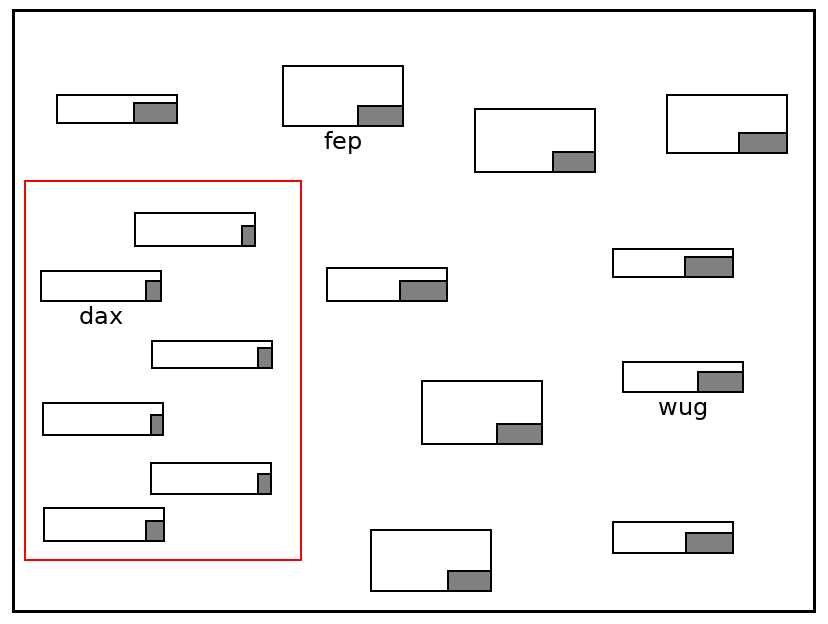
\includegraphics[width=0.7\textwidth]{figures/semi-supervised-demo.png}
    \caption{Screenshot from the task illustrating the stimuli and labels used in the experiment (this example is from the {\sc distinct structure} and {\sc distinct labels} condition). In all conditions, people were asked to sort the rectangles into categories by dragging them around the screen into clusters. In this screenshot the participant has already drawn one box around one of the categories they identified.}
    \label{experiment-demo}
  \end{center}
\end{figure}

\subsection{Design}

Participants were randomly assigned to conditions based on two between-subject manipulations. In the first, we varied the coherence of the underlying category structure. In the \textsc{distinct structure} condition, the stimuli consisted of three well-separated clusters that varied along both stimulus dimensions, as shown in the top row of Figure~\ref{experiment-conditions}. The \textsc{ambiguous structure} condition also consisted of three equally sized clusters, but they were much closer together in the stimulus space, as in the bottom row of Figure~\ref{experiment-conditions}. This made it difficult to distinguish the cluster boundaries from feature information alone. In all conditions the participants were not told how many categories there were: they were instructed to sort the stimuli into as many categories as they felt was necessary.

\begin{figure*}[t]
  \begin{center}
    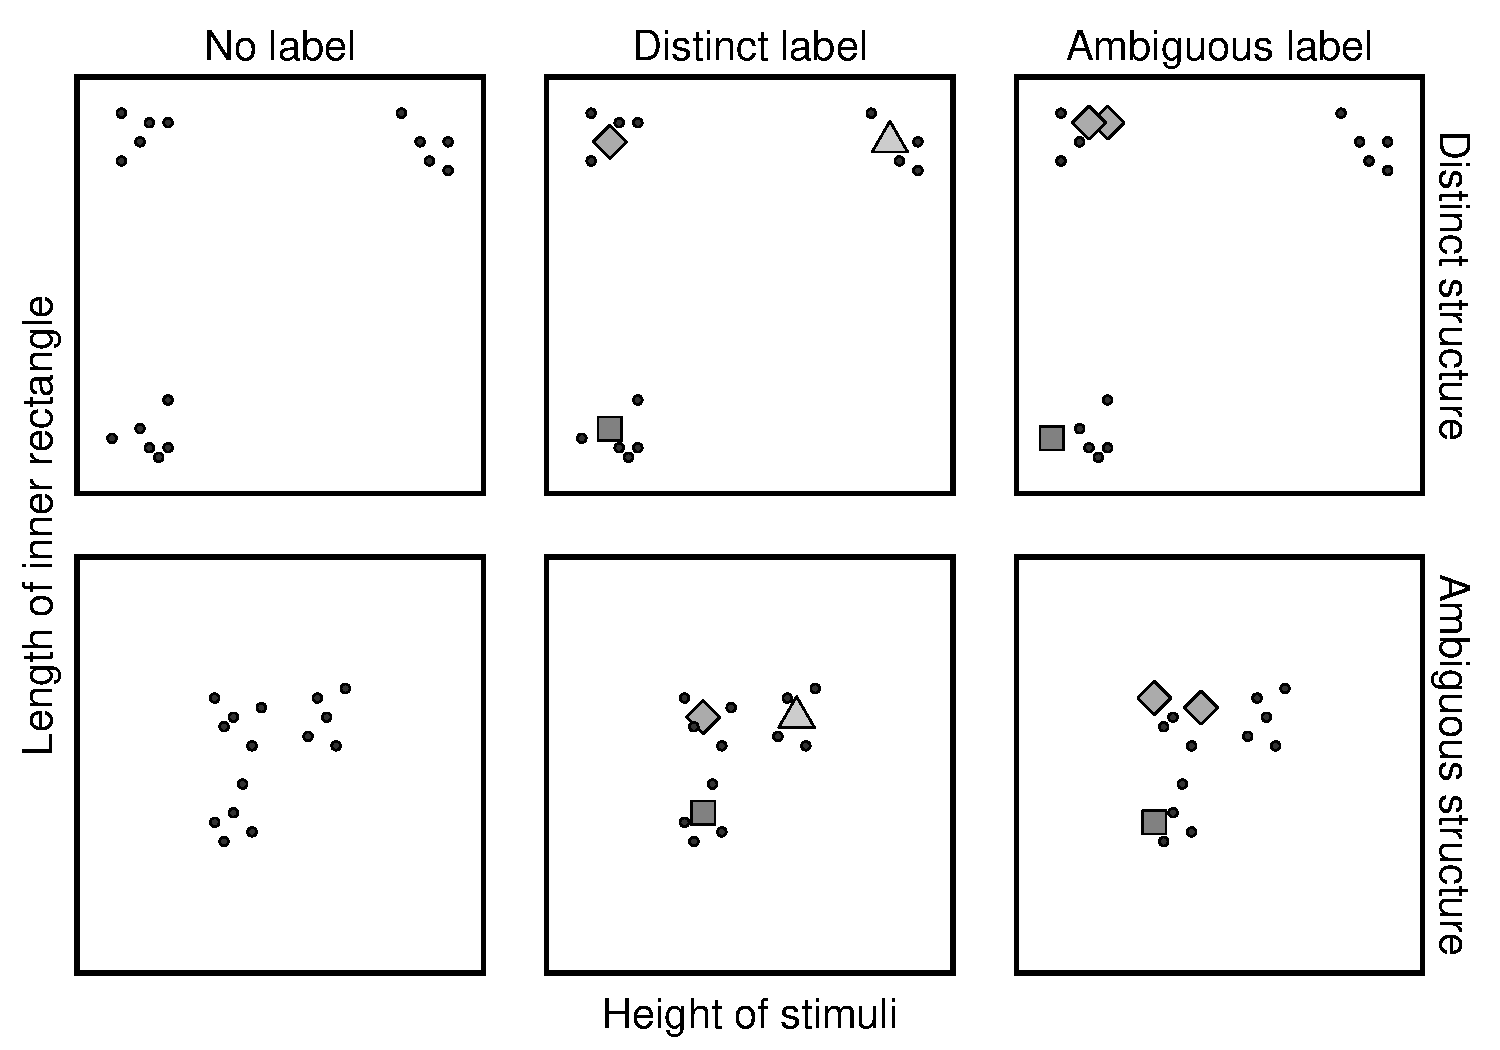
\includegraphics[width=0.8\textwidth]{figures/category-structures.pdf}
    \caption{A visualization of the experimental design. The stimuli varied along two continuous dimensions (stimuli height and the length of the inner rectangle). The small black dots represent the unlabeled examples, while the larger stimuli represent the labeled examples, with each shape corresponding to a different category label ({\it dax}, {\it wug} or {\it fep}).}
    \label{experiment-conditions}
  \end{center}
\end{figure*}

The second experimental manipulation, shown in the columns of Figure~\ref{experiment-conditions}, varied the informativeness of the labels that were included. As a baseline, the \textsc{no label} condition was fully unsupervised with no labels at all. In the \textsc{distinct label} condition, people saw a helpful and informative set of labels: one labeled example from each of the three clusters. By contrast, in the \textsc{ambiguous label} condition people saw potentially misleading labels: one came from the first cluster, two came from the second cluster, and none came from the third cluster. Of interest is how people's categorizations were affected by the informativeness of the label in combination with the structural coherence in the unsupervised data.

\subsection{Procedure}

The experiment was run online through a custom website. The cover story informed participants that archaeologists had discovered a number of unknown objects on a recent expedition, and needed help to sort them into different categories. In the labeled conditions participants were told that the archaeologists had discovered some of the names of the objects, which could be used as a guide on how they sorted the stimuli. In the {\sc no label} condition the instructions simply recommended using the appearance of the objects to guide the sorting. In all conditions, no indication was given of how many different categories were present in the data.

In order to make sure that people understood the sorting task, before beginning the main task the participants completed a demonstration trial. This trial contained three squares and three triangles of different sizes, where they were asked to sort the shapes into separate piles that they thought should naturally go together. The position of objects in both the demonstration trial and main task were arranged to be non-overlapping and randomly ordered for each participant. The user interface required participants to first click and drag on stimuli until they were sorted into piles they thought should belong together, and then to draw boxes around each pile. If people were unhappy with the boxes they could revert to the click and drag stage until they were satisfied. If anyone failed to group any stimuli inside a box or assigned any stimuli to multiple boxes, a warning would appear and they could not submit their response. The demonstration trial also served as an exclusion criterion: 52 people failed to sort those stimuli in a sensible way (i.e., not by size or shape) and their data from the main experiment were therefore excluded from further analysis.

\section{Results}

\begin{figure*}[t]
  \begin{center}
    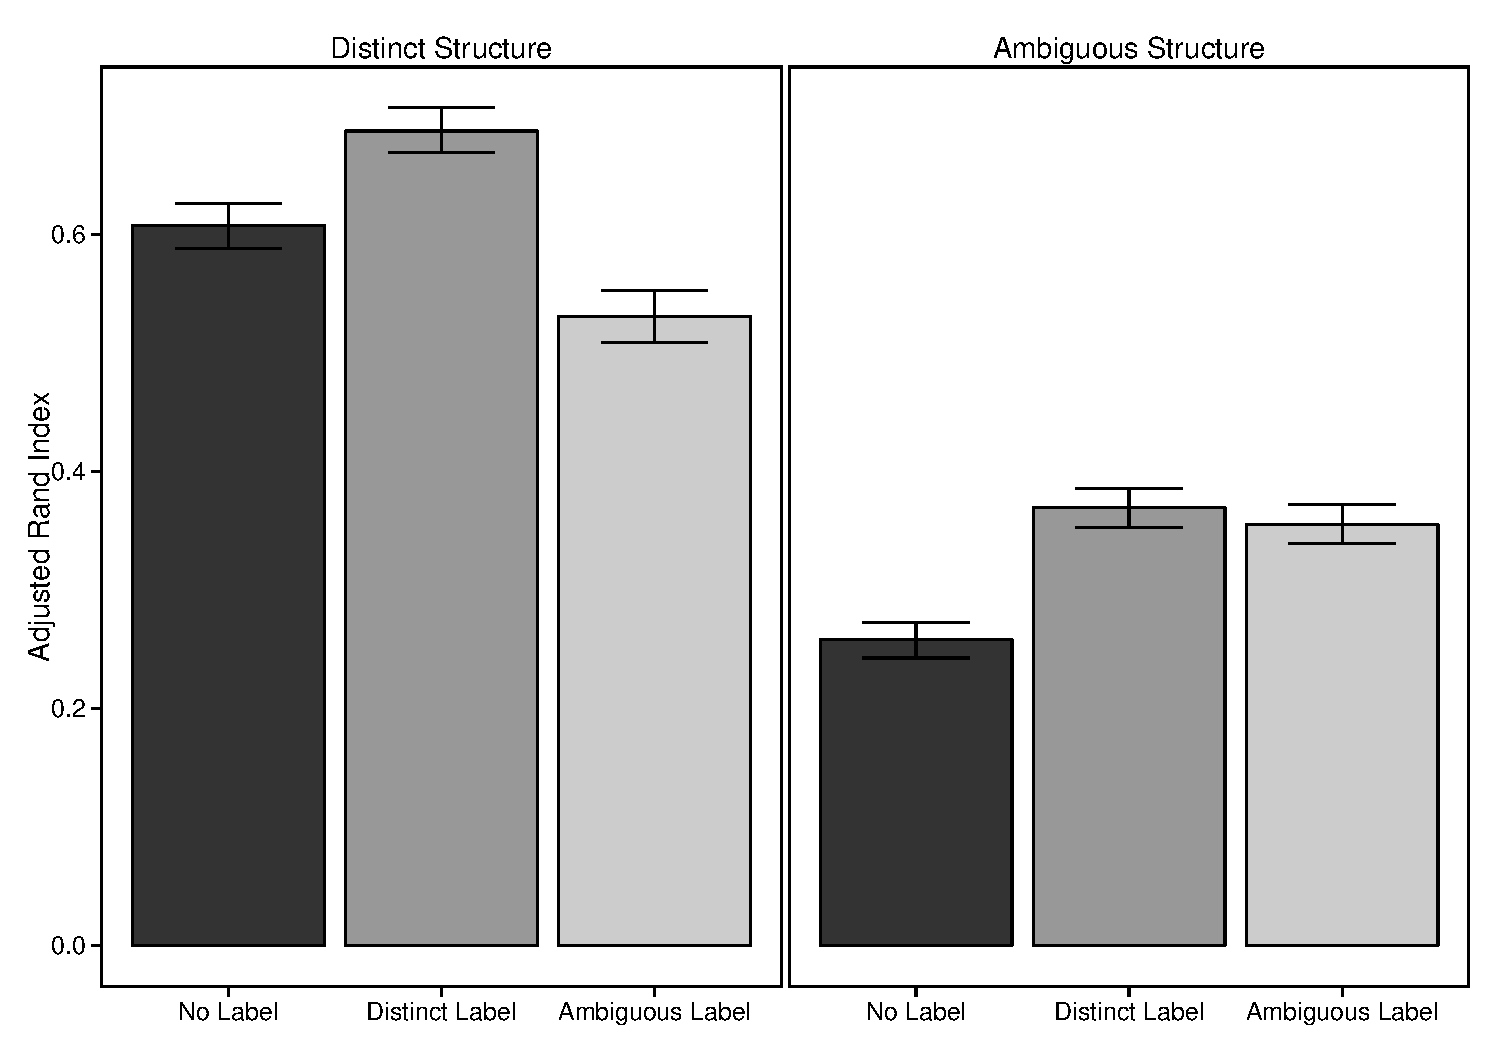
\includegraphics[width=0.9\textwidth]{figures/adjR-comparison-means.pdf}
    \caption{Agreement between participants within condition. Each bar plots the average similarity between solutions (i.e., adjusted Rand index) taken across all subjects in the same condition. Error bars are bootstrapped 95\% confidence intervals.}
    \label{adjr-comparison-means}
  \end{center}
\end{figure*}

Participants produced 216 unique sorts out of 504 solutions analyzed. This level of variability is commensurate with similar tasks in unsupervised categorization \cite<e.g.>{pothos2011measuring}. However, the extent of the variability was very different across conditions. To quantify this variability we use the adjusted Rand index (\textit{adjR}), which measures the similarity between two classifications \cite{hubert1985comparing}. It has a maximum of one when both classifications are the same, and drops to zero if the agreement between them is no more than would be expected by chance. The average \textit{adjR} score among all pairs of participants in each condition is shown in Figure \ref{adjr-comparison-means}, and reveals two key findings.

The first finding was that people did indeed appear to find the ambiguous structure more ambiguous: responses in the \textsc{distinct structure} condition were more similar to one another than those in the \textsc{ambiguous structure} condition. Consistent with this, a two-way ANOVA on structure \(\times\) label revealed a significant main effect of structure (\textit{F}(1, 498) = 293.5, \textit{p} < 0.001).

The second finding, of more importance, is that the effect of labels was different in different contexts: while there was a significant main effect of label (\textit{F}(2, 498) = 14.2, \textit{p} < 0.001), there was also a significant interaction between the structure condition and label condition (\textit{F}(2, 498) = 10.9, \textit{p} < 0.001). In the \textsc{ambiguous structure} condition, adding labels increased the degree of agreement among participants regardless of which label set was provided. However, in the \textsc{distinct structure} condition, the effect was more subtle. When the \textsc{distinct labels} were provided, the labeled data were consistent with the structure of the unlabeled data, and the agreement among participants increased relative to the \textsc{no label} condition. But when the \textsc{ambiguous labels} were provided, the structure among the labeled examples did not precisely match the structure of the unlabeled data. As a result, the agreement among participants dropped relative to the \textsc{no label} condition.


\begin{figure*}[t]
  \begin{center}
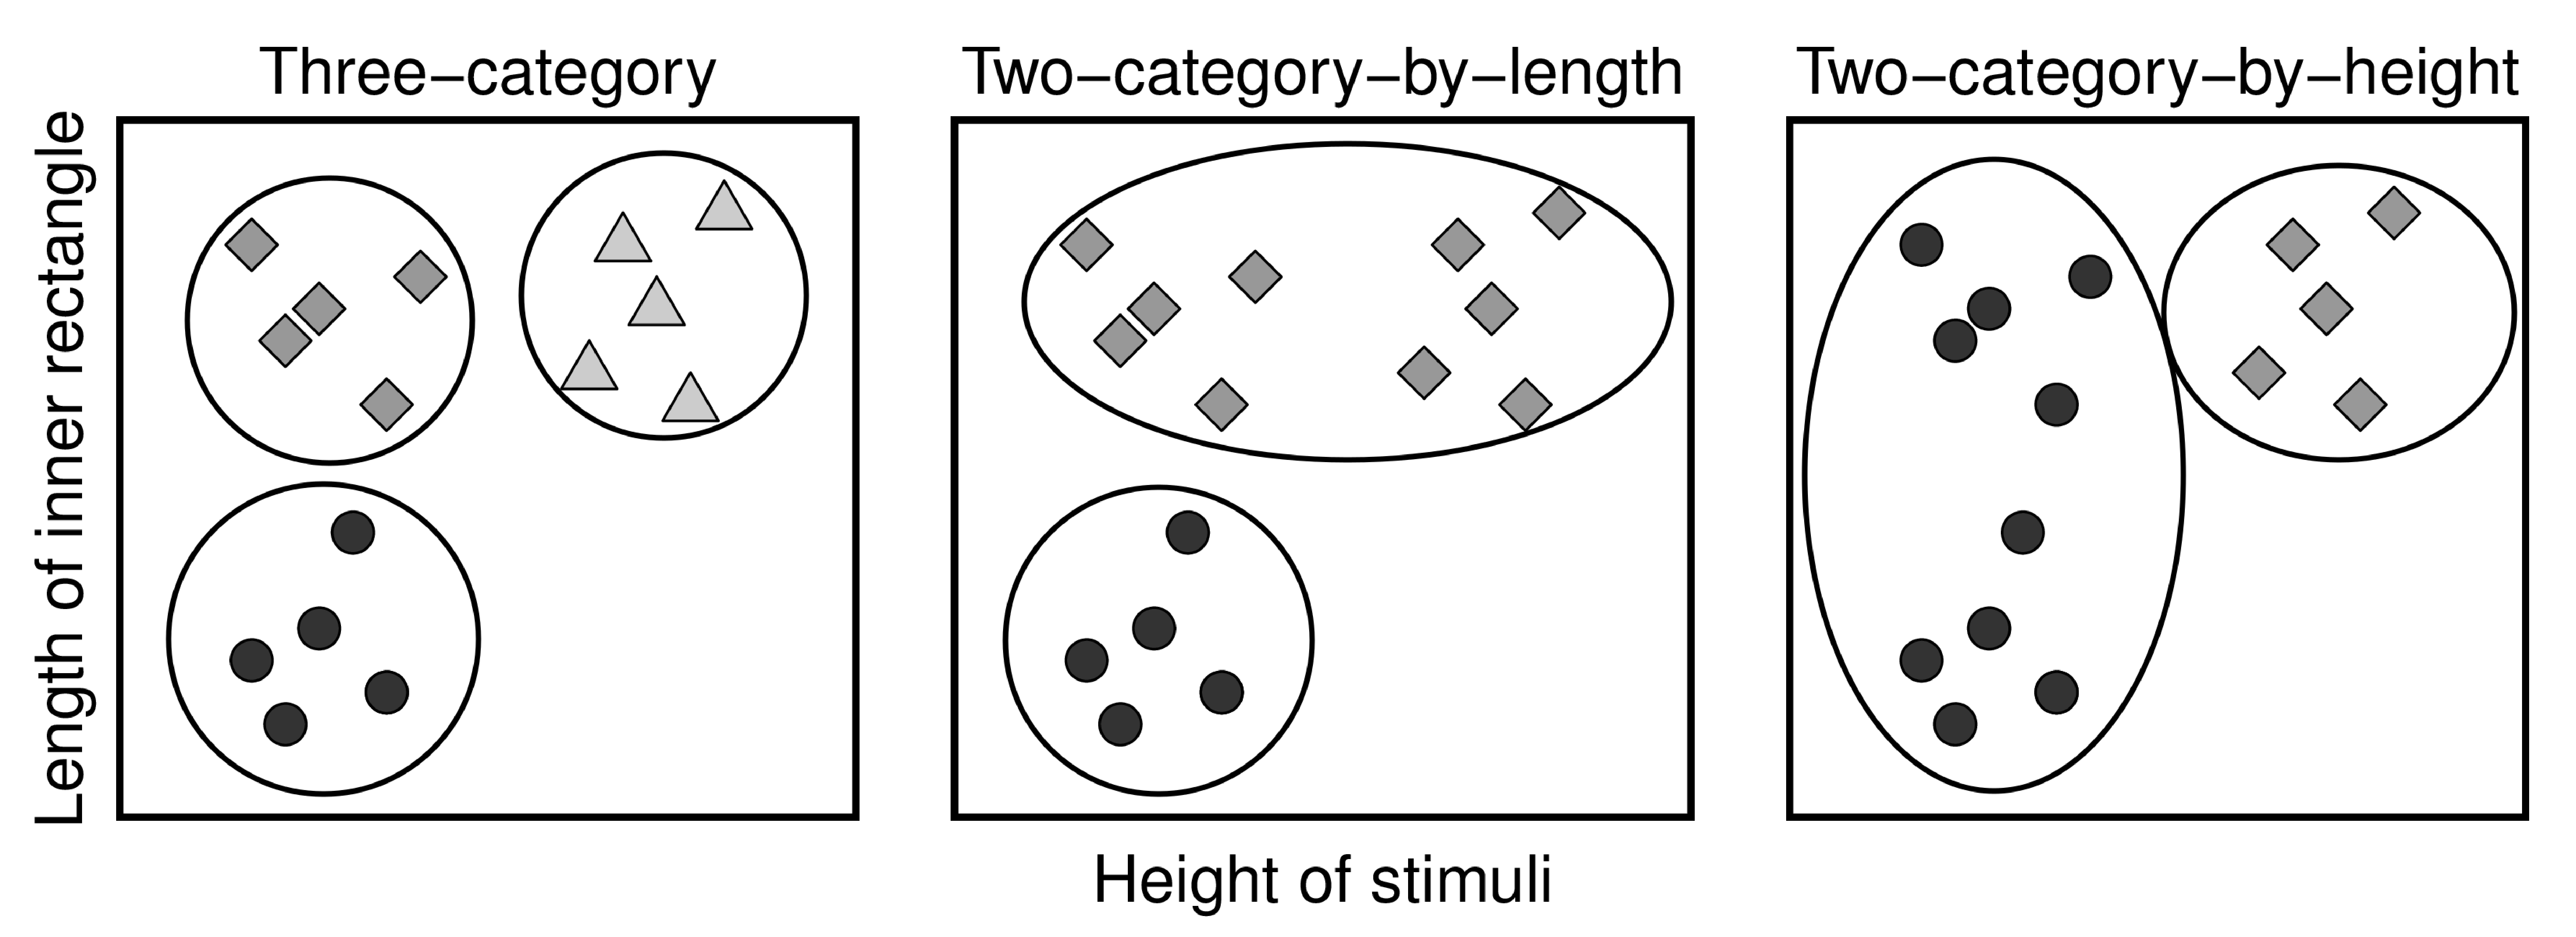
\includegraphics[width=0.8\textwidth]{figures/canonical-strategies-two.pdf}
    \caption{The three canonical classifications used to classify people's responses in the task. While this figure only depicts the canonical classifications for the \textsc{ambiguous structure} condition, the strategies are analogous for the \textsc{distinct structure} condition. The three-category strategy required attending to both stimulus dimensions when sorting. On the other hand, the two-category-by-length and two-category-by-height strategies only required attending to a single stimulus dimension corresponding to either the length of the inner rectangle or the height of the stimuli respectively.}
    \label{canonical-classifications}
  \end{center}
\end{figure*}

On close inspection it turns out that most answers were variants\footnote{It was not unusual for a participant to classify {\it most} of the stimuli according to one of these schemes, with some of the boundary cases being different; situations like this meant that 187 of the 216 distinct unique sorts were only produced by a single participant.} of one of the three classification schemes shown in Figure \ref{canonical-classifications}, which we refer to as the three ``canonical classifications'' for the task. Participants almost always approximately (a) sorted into three categories using both stimulus dimensions, (b) sorted into two categories based on height, or (c) sorted into two categories based on length.
We assigned people to one of the three classifications by calculating the {\it adjR} value between each person's sort and each of the three canonical classifications, and then selected the one that was highest as their classification strategy.\footnote{We also ran analyses in which we grouped participants into an ``other'' strategy if their solutions were insufficiently similar to any of the canonical classifications (e.g. having {\it adjR} values below a certain threshold like 0.2 for all three canonical classifications). The qualitative pattern of results remains unchanged across different threshold values ranging from 0.1 to 0.5.}
The breakdown of classification type by condition is shown in the top row of Figure \ref{strategy-histogram}.

In the  \textsc{distinct structure} condition the results were straightforward. The choice of labeling scheme had no effect on the classification strategy (\(\chi^2(4) = 1.90, p = 0.75\)) and participants tended to use the three category solution regardless of the nature of the labels. Even when one cluster of stimuli was given no labels at all, as in the \textsc{ambiguous label} condition, people detected the unlabeled cluster and did not attempt to group those items with items in the labeled clusters. This suggests that if the category structure is coherent and obvious enough, labels make very little difference to people's categorizations.

For the \textsc{ambiguous structure} condition the story is more complex, and there is a significant difference in classifications depending on the nature of the labels shown (\(\chi^2(4) = 26.48, p < 0.001\)).\footnote{Significant differences were also observed between each pair of label conditions (\textsc{no label} and \textsc{distinct label}: \(\chi^2(2) = 10.47, p < .01\), \textsc{no label} and \textsc{ambiguous labels}: \(\chi^2(2) = 15.61, p < .01\) and \textsc{distinct labels} and \textsc{ambiguous labels}: \(\chi^2(2) = 12.69, p < .01\)).} In the \textsc{no label} condition, people were evenly split between the three classification schemes. This reflects the fact that the raw stimulus information was not sufficient for people to infer how to categorize the items. When labels were provided, participants relied on them heavily. In the \textsc{distinct label} condition people preferred the three category solution, since the labeling scheme explicitly picked out the three clusters. In the \textsc{ambiguous label} condition, the labels ruled out the two-category-by-height strategy, but did not distinguish between the other two strategies. This is reflected in the data, with people split evenly between the three-category and two-category-by-length strategies.


\begin{figure*}[t]
  \begin{center}
    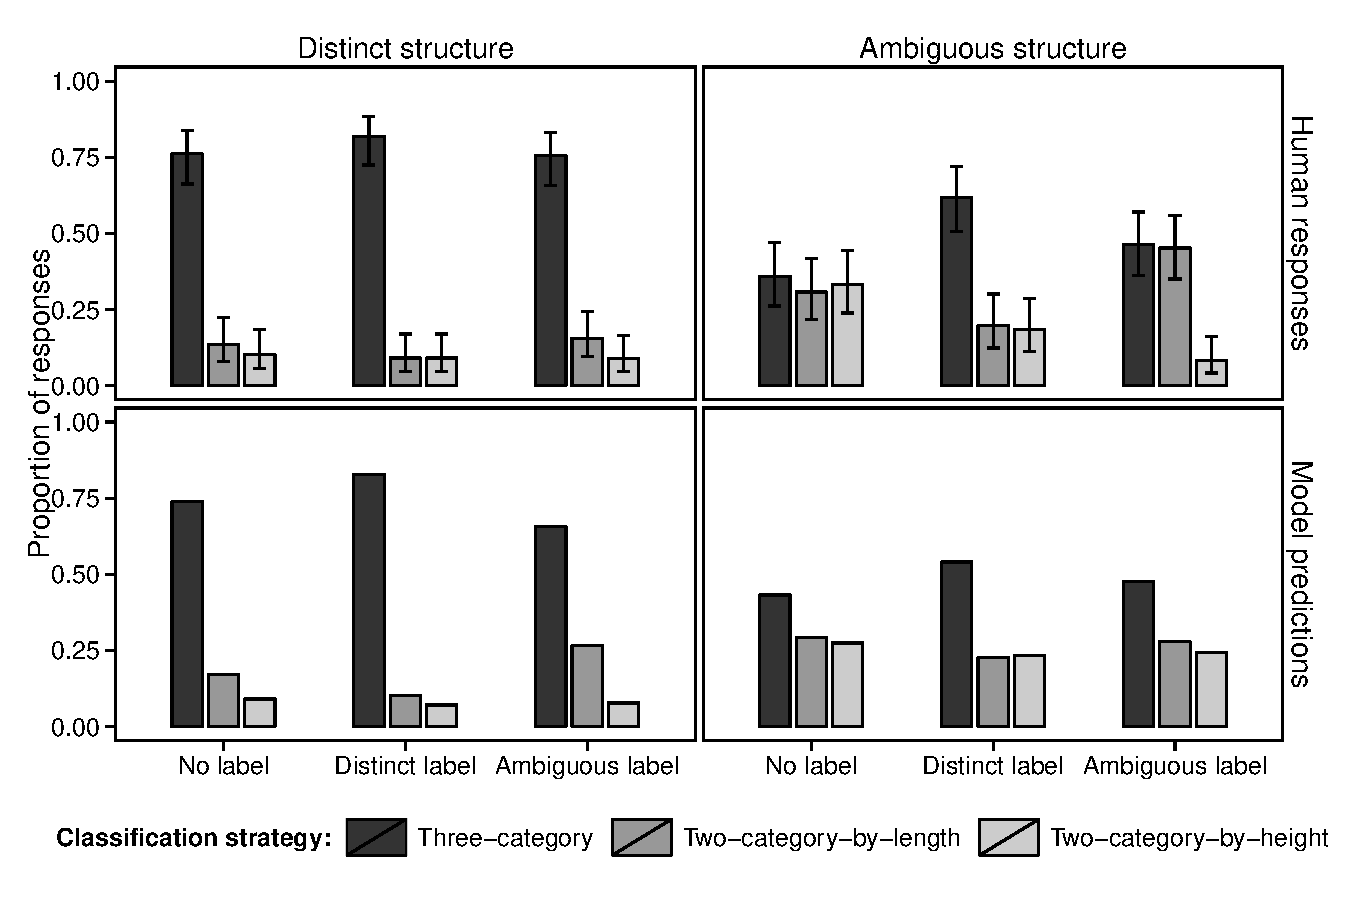
\includegraphics[width=1\textwidth]{figures/human-model-strategies.pdf}
    \caption{Comparison between the proportion of strategies used by humans and predicted by the Rational model across each of the experimental conditions. Error bars plot 95\% confidence intervals for the human responses. People in the \textsc{distinct structure} mostly relied on unlabeled information, with labeled examples having little effect in their choice of classification strategy. In contrast, there was a strong effect in how labels were used by people in the \textsc{ambiguous structure} conditions. The rational model of categorization captures people's responses reasonably well in both conditions.}
    \label{strategy-histogram}
  \end{center}
\end{figure*}

Although the overall pattern of results is a complicated interaction between stimulus structure and labeling scheme, the interpretation of this interaction effect is simple. When the stimulus structure was unambiguous, providing additional labeled data had no influence on how people learned. In such cases semi-supervised learning looks the same as unsupervised learning. In contrast, when the stimulus structure was ambiguous, even a very small number of labeled examples had a big impact on how people learned, pushing people towards one solution or another depending on the information provided by the labels.


\section{Model fitting}

It appears that people produced sensible behavior in this task, but one question remains: can we account for this performance based on standard psychological theories of categorization, or is it necessary to postulate entirely different mechanisms or abilities? To address this question, we applied a modified version of Anderson's \citeyear{anderson1991adaptive} Rational Model of Categorization (RMC) to the task. The RMC is a Bayesian category learning model that has previously been applied to a variety of tasks in supervised learning \cite{anderson1991adaptive}, unsupervised learning \cite{clapper2002adaptive, pothos2011measuring} and semi-supervised learning \cite{zhu2010cognitive}. We chose to focus on the RMC because it lends itself well to the situation our participants were in: it assumes that stimuli belong to one of several categories, but does not know how many categories exist and so attempts to infer this from the data. However, there is no inherent reason why other successful category learning models such as SUSTAIN \cite{love2004sustain} could not also be similarly adapted. The RMC learns the number of categories by relying on a simple sequential assignment method known as the Chinese restaurant process, which specifies the prior probability of a particular category (proportional to the number of items in that category) and the prior probability of a new category (a constant). For a detailed discussion of the RMC in the form we implemented it, see \citeA{sanborn2010rational}.

It was necessary to modify the RMC slightly in order to apply to this task.  A critical feature of the RMC is that category labels are viewed as an additional feature possessed by stimuli. From this perspective our task involves two continuous features (height and length) and one discrete one (label). A category is associated with a probability distribution over all three features. In Anderson's \citeyear{anderson1991adaptive} formulation, the number of possible values that a discrete feature can take is assumed to be known in advance.
In our task this assumption is inappropriate, since the number of possible labels is not known to the learner. Fortunately this is easy to rectify: we assume that the distribution over labels is itself sampled from a Chinese restaurant process, consistent with the prior distribution over category assignments. Thus, labels of the same type would tend to belong to the same clusters, while items with unseen labels would be more likely to be assigned to new clusters.

Each run of the RMC outputs a set of category assignments for the observed stimuli (directly analogous to the responses we collected from participants). This output was compared to human responses by applying the same procedure that we applied to the human data: assigning each classification to one of the three canonical strategies based on the {\it adjR} index. Results for each condition reflect 5000 independent runs, with the order that the stimuli were presented to the model randomized between runs.

The output of the RMC, plotted in the bottom row of Figure \ref{strategy-histogram}, is qualitatively consistent with the pattern of responses produced by human subjects. For example, in the \textsc{distinct structure} conditions, the model predicted that the three category classification would be preferred regardless of the nature of the labels. It also predicted, similarly to people, greater variation in the strategies in the \textsc{ambiguous structure} conditions. There were a few cases where the model predictions did not exactly match the responses given by people, most notably in the \textsc{ambiguous structure, ambiguous label} condition, where it did not rule out the two category by height classification like people did.\footnote{The model's responses in this condition suggest that this result is driven primarily by runs where it did not observe the labeled instances necessary for correct classification until near the end of the run.}

Overall, the correlation between the predictions of the modified RMC and the data from participants in the proportion of responses for each strategy was 0.92. This suggests that despite its imperfections, the RMC is able to roughly reproduce human performance for a novel semi-supervised task.  Given that this is the first study that we are aware of that tries to compare semi-supervised learning to unsupervised learning (rather than to supervised learning) and where the number of labels is not known, it is reassuring to see that existing theory generalizes well to this situation.

\section{Discussion}

Most of the literature on semi-supervised learning takes supervised learning as its starting point, and examines the extent to which additional unlabeled data shifts people's learned category representations relative to people only presented only with labeled data. The results in this area have been mixed, with studies finding that in some situations unlabeled data has an effect in semi-supervised learning \cite{zhu2007humans, lake2011estimating, kalish2011can} and in others where it does not \cite{mcdonnell2012sparse}. Our work adopts a very different framing of the semi-supervised learning problem: instead of asking how semi-supervised learning differs from supervised learning, we ask how it differs from unsupervised learning. Instead of asking when unlabeled data have an influence on learning, we investigate when labeled data are helpful.

Our core results bear a superficial similarity to previous work, insofar as our key finding is that labeled data is sometimes helpful, and sometimes it has no effect on learning. However, our experimental manipulations make it clear when and why it happens. When the unlabeled data is informative enough that the category structure is unambiguous, people do not need labeled data to guide learning. As \citeA{bloom2002children} suggests, semi-supervised learning appears indistinguishable from unsupervised learning in this scenario. In contrast, when the unlabeled data is ambiguous, labels become more powerful and have a large effect on the categories that people infer -- in this case, the specific set of labels shown helps people determine which dimensions are relevant for classification. This includes whether to stick with a simpler unidimensional strategy or to switch to a more complex multi-dimensional classification strategy. Of course, ambiguous situations may not be the only kind of instance where labeled examples are useful. The results from \citeA{vandist2009semisupervised} suggest that labeled examples can also help in learning complex Information-Integration categories -- in that case, the categories are well-separated and not ambiguous but still require integrating information from multiple dimensions.

The historical prevalence of supervised learning as a topic of interest in cognitive science and machine learning has implicitly taken supervised learning to be the natural reference point against which semi-supervised learning should be assessed. In our view, this assumption also reflects an incomplete view of human semi-supervised learning. The category learning problems people -- especially children -- face in real life do not usually involve a few unlabeled examples in addition to many labeled ones. Rather, the world naturally presents people with a rich distribution of unlabeled data, which helpful teachers (such as parents) supplement by labeling.

Comparing semi-supervised learning to unsupervised learning sheds light on the critical role that labeled data plays in human learning. In particular, much of the difficulty in how humans learn categories is in the unsupervised aspects of determining how things should be grouped together. Here we argue that labels play a fundamental part in making sense of it, especially when the categories are ambiguous without them. It is an open question to what extent categories in the natural world are ambiguous in this way. Future work should investigate cases where labeled examples are informative in other ways, such as when objects belong to multiple cross-cutting categories \cite{shafto2011probabilistic} or when items organized into taxonomies have multiple labels \cite{canini2011nonparametric}.

\section{Acknowledgments}

Correspondence concerning this article should be addressed to Wai Keen Vong, School of Psychology, University of Adelaide SA 5005, Australia (waikeen.vong@adelaide.edu.au). Daniel J. Navarro received salary support from Australian Research Council grant FT110100431 and Amy Perfors from Australian Research Council grant DE120102378. Research costs were funded through Australian Research Council grant DP110104949.

%\bibliographystyle{apacite}
%\nocite{*}
%\bibliography{vong_perfors_navarro_semisupervised_learning}

\begin{thebibliography}{}

\bibitem [\protect \citeauthoryear {%
Anderson%
}{%
Anderson%
}{%
{\protect \APACyear {1991}}%
}]{%
anderson1991adaptive}
\APACinsertmetastar {%
anderson1991adaptive}%
\begin{APACrefauthors}%
Anderson, J\BPBI R.%
\end{APACrefauthors}%
\unskip\
\newblock
\APACrefYearMonthDay{1991}{}{}.
\newblock
{\BBOQ}\APACrefatitle {The adaptive nature of human categorization.} {The
  adaptive nature of human categorization.}{\BBCQ}
\newblock
\APACjournalVolNumPages{Psychological Review}{98}{3}{409--429}.
\PrintBackRefs{\CurrentBib}

\bibitem [\protect \citeauthoryear {%
Ashby%
, Queller%
\BCBL {}\ \BBA {} Berretty%
}{%
Ashby%
\ \protect \BOthers {.}}{%
{\protect \APACyear {1999}}%
}]{%
ashby1999dominance}
\APACinsertmetastar {%
ashby1999dominance}%
\begin{APACrefauthors}%
Ashby, F\BPBI G.%
, Queller, S.%
\BCBL {}\ \BBA {} Berretty, P\BPBI M.%
\end{APACrefauthors}%
\unskip\
\newblock
\APACrefYearMonthDay{1999}{}{}.
\newblock
{\BBOQ}\APACrefatitle {On the dominance of unidimensional rules in unsupervised
  categorization} {On the dominance of unidimensional rules in unsupervised
  categorization}.{\BBCQ}
\newblock
\APACjournalVolNumPages{Perception \& Psychophysics}{61}{6}{1178--1199}.
\PrintBackRefs{\CurrentBib}

\bibitem [\protect \citeauthoryear {%
Bloom%
}{%
Bloom%
}{%
{\protect \APACyear {2000}}%
}]{%
bloom2002children}
\APACinsertmetastar {%
bloom2002children}%
\begin{APACrefauthors}%
Bloom, P.%
\end{APACrefauthors}%
\unskip\
\newblock
\APACrefYear{2000}.
\newblock
\APACrefbtitle {How children learn the meaning of words} {How children learn
  the meaning of words}.
\newblock
\APACaddressPublisher{Cambridge, MA}{MIT Press}.
\PrintBackRefs{\CurrentBib}

\bibitem [\protect \citeauthoryear {%
Bruner%
, Goodnow%
\BCBL {}\ \BBA {} Austin%
}{%
Bruner%
\ \protect \BOthers {.}}{%
{\protect \APACyear {1956}}%
}]{%
bruner1956study}
\APACinsertmetastar {%
bruner1956study}%
\begin{APACrefauthors}%
Bruner, J\BPBI S.%
, Goodnow, J\BPBI J.%
\BCBL {}\ \BBA {} Austin, G\BPBI A.%
\end{APACrefauthors}%
\unskip\
\newblock
\APACrefYear{1956}.
\newblock
\APACrefbtitle {A study of thinking} {A study of thinking}.
\newblock
\APACaddressPublisher{New York}{John Wiley and Sons}.
\PrintBackRefs{\CurrentBib}

\bibitem [\protect \citeauthoryear {%
Canini%
\ \BBA {} Griffiths%
}{%
Canini%
\ \BBA {} Griffiths%
}{%
{\protect \APACyear {2011}}%
}]{%
canini2011nonparametric}
\APACinsertmetastar {%
canini2011nonparametric}%
\begin{APACrefauthors}%
Canini, K\BPBI R.%
\BCBT {}\ \BBA {} Griffiths, T\BPBI L.%
\end{APACrefauthors}%
\unskip\
\newblock
\APACrefYearMonthDay{2011}{}{}.
\newblock
{\BBOQ}\APACrefatitle {A Nonparametric Bayesian Model of Multi-Level Category
  Learning.} {A nonparametric bayesian model of multi-level category
  learning.}{\BBCQ}
\newblock
\BIn{} \APACrefbtitle {{Proceedings of the 25th AAAI Conference on Artificial
  Intelligence}.} {{Proceedings of the 25th AAAI Conference on Artificial
  Intelligence}.}
\PrintBackRefs{\CurrentBib}

\bibitem [\protect \citeauthoryear {%
Chapelle%
, Sch{\"o}lkopf%
\BCBL {}\ \BBA {} Zien%
}{%
Chapelle%
\ \protect \BOthers {.}}{%
{\protect \APACyear {2006}}%
}]{%
chapelle2006semi}
\APACinsertmetastar {%
chapelle2006semi}%
\begin{APACrefauthors}%
Chapelle, O.%
, Sch{\"o}lkopf, B.%
\BCBL {}\ \BBA {} Zien, A.%
\end{APACrefauthors}%
\unskip\
\newblock
\APACrefYear{2006}.
\newblock
\APACrefbtitle {Semi-supervised learning} {Semi-supervised learning}\
  (\BVOL~2).
\newblock
\APACaddressPublisher{}{MIT press Cambridge}.
\PrintBackRefs{\CurrentBib}

\bibitem [\protect \citeauthoryear {%
Clapper%
\ \BBA {} Bower%
}{%
Clapper%
\ \BBA {} Bower%
}{%
{\protect \APACyear {2002}}%
}]{%
clapper2002adaptive}
\APACinsertmetastar {%
clapper2002adaptive}%
\begin{APACrefauthors}%
Clapper, J\BPBI P.%
\BCBT {}\ \BBA {} Bower, G\BPBI H.%
\end{APACrefauthors}%
\unskip\
\newblock
\APACrefYearMonthDay{2002}{}{}.
\newblock
{\BBOQ}\APACrefatitle {Adaptive categorization in unsupervised learning.}
  {Adaptive categorization in unsupervised learning.}{\BBCQ}
\newblock
\APACjournalVolNumPages{Journal of Experimental Psychology: Learning, Memory,
  and Cognition}{28}{5}{908}.
\PrintBackRefs{\CurrentBib}

\bibitem [\protect \citeauthoryear {%
Gibson%
, Rogers%
\BCBL {}\ \BBA {} Zhu%
}{%
Gibson%
\ \protect \BOthers {.}}{%
{\protect \APACyear {2013}}%
}]{%
gibson2013human}
\APACinsertmetastar {%
gibson2013human}%
\begin{APACrefauthors}%
Gibson, B\BPBI R.%
, Rogers, T\BPBI T.%
\BCBL {}\ \BBA {} Zhu, X.%
\end{APACrefauthors}%
\unskip\
\newblock
\APACrefYearMonthDay{2013}{}{}.
\newblock
{\BBOQ}\APACrefatitle {Human Semi-Supervised Learning} {Human semi-supervised
  learning}.{\BBCQ}
\newblock
\APACjournalVolNumPages{Topics in Cognitive Science}{5}{1}{132--172}.
\PrintBackRefs{\CurrentBib}

\bibitem [\protect \citeauthoryear {%
Hubert%
\ \BBA {} Arabie%
}{%
Hubert%
\ \BBA {} Arabie%
}{%
{\protect \APACyear {1985}}%
}]{%
hubert1985comparing}
\APACinsertmetastar {%
hubert1985comparing}%
\begin{APACrefauthors}%
Hubert, L.%
\BCBT {}\ \BBA {} Arabie, P.%
\end{APACrefauthors}%
\unskip\
\newblock
\APACrefYearMonthDay{1985}{}{}.
\newblock
{\BBOQ}\APACrefatitle {Comparing partitions} {Comparing partitions}.{\BBCQ}
\newblock
\APACjournalVolNumPages{{Journal of Classification}}{2}{1}{193--218}.
\PrintBackRefs{\CurrentBib}

\bibitem [\protect \citeauthoryear {%
Kalish%
, Rogers%
, Lang%
\BCBL {}\ \BBA {} Zhu%
}{%
Kalish%
\ \protect \BOthers {.}}{%
{\protect \APACyear {2011}}%
}]{%
kalish2011can}
\APACinsertmetastar {%
kalish2011can}%
\begin{APACrefauthors}%
Kalish, C\BPBI W.%
, Rogers, T\BPBI T.%
, Lang, J.%
\BCBL {}\ \BBA {} Zhu, X.%
\end{APACrefauthors}%
\unskip\
\newblock
\APACrefYearMonthDay{2011}{}{}.
\newblock
{\BBOQ}\APACrefatitle {Can semi-supervised learning explain incorrect beliefs
  about categories?} {Can semi-supervised learning explain incorrect beliefs
  about categories?}{\BBCQ}
\newblock
\APACjournalVolNumPages{Cognition}{120}{1}{106--118}.
\PrintBackRefs{\CurrentBib}

\bibitem [\protect \citeauthoryear {%
Lake%
\ \BBA {} McClelland%
}{%
Lake%
\ \BBA {} McClelland%
}{%
{\protect \APACyear {2011}}%
}]{%
lake2011estimating}
\APACinsertmetastar {%
lake2011estimating}%
\begin{APACrefauthors}%
Lake, B.%
\BCBT {}\ \BBA {} McClelland, J.%
\end{APACrefauthors}%
\unskip\
\newblock
\APACrefYearMonthDay{2011}{}{}.
\newblock
{\BBOQ}\APACrefatitle {Estimating the strength of unlabeled information during
  semi-supervised learning} {Estimating the strength of unlabeled information
  during semi-supervised learning}.{\BBCQ}
\newblock
\BIn{} \APACrefbtitle {{Proceedings of the 33rd Annual Conference of the
  Cognitive Science Society}} {{Proceedings of the 33rd Annual Conference of
  the Cognitive Science Society}}\ (\BPGS\ 1400--1405).
\PrintBackRefs{\CurrentBib}

\bibitem [\protect \citeauthoryear {%
Lewis%
\ \BBA {} Frank%
}{%
Lewis%
\ \BBA {} Frank%
}{%
{\protect \APACyear {2013}}%
}]{%
lewis2013integrated}
\APACinsertmetastar {%
lewis2013integrated}%
\begin{APACrefauthors}%
Lewis, M.%
\BCBT {}\ \BBA {} Frank, M\BPBI C.%
\end{APACrefauthors}%
\unskip\
\newblock
\APACrefYearMonthDay{2013}{}{}.
\newblock
{\BBOQ}\APACrefatitle {An integrated model of concept learning and word-concept
  mapping} {An integrated model of concept learning and word-concept
  mapping}.{\BBCQ}
\newblock
\BIn{} \APACrefbtitle {{Proceedings of the 35th Annual Conference of the
  Cognitive Science Society}.} {{Proceedings of the 35th Annual Conference of
  the Cognitive Science Society}.}
\PrintBackRefs{\CurrentBib}

\bibitem [\protect \citeauthoryear {%
Love%
}{%
Love%
}{%
{\protect \APACyear {2002}}%
}]{%
love2002comparing}
\APACinsertmetastar {%
love2002comparing}%
\begin{APACrefauthors}%
Love, B\BPBI C.%
\end{APACrefauthors}%
\unskip\
\newblock
\APACrefYearMonthDay{2002}{}{}.
\newblock
{\BBOQ}\APACrefatitle {Comparing supervised and unsupervised category learning}
  {Comparing supervised and unsupervised category learning}.{\BBCQ}
\newblock
\APACjournalVolNumPages{Psychonomic Bulletin \& Review}{9}{4}{829--835}.
\PrintBackRefs{\CurrentBib}

\bibitem [\protect \citeauthoryear {%
Love%
, Medin%
\BCBL {}\ \BBA {} Gureckis%
}{%
Love%
\ \protect \BOthers {.}}{%
{\protect \APACyear {2004}}%
}]{%
love2004sustain}
\APACinsertmetastar {%
love2004sustain}%
\begin{APACrefauthors}%
Love, B\BPBI C.%
, Medin, D\BPBI L.%
\BCBL {}\ \BBA {} Gureckis, T\BPBI M.%
\end{APACrefauthors}%
\unskip\
\newblock
\APACrefYearMonthDay{2004}{}{}.
\newblock
{\BBOQ}\APACrefatitle {SUSTAIN: a network model of category learning.}
  {Sustain: a network model of category learning.}{\BBCQ}
\newblock
\APACjournalVolNumPages{Psychological review}{111}{2}{309}.
\PrintBackRefs{\CurrentBib}

\bibitem [\protect \citeauthoryear {%
McDonnell%
, Jew%
\BCBL {}\ \BBA {} Gureckis%
}{%
McDonnell%
\ \protect \BOthers {.}}{%
{\protect \APACyear {2012}}%
}]{%
mcdonnell2012sparse}
\APACinsertmetastar {%
mcdonnell2012sparse}%
\begin{APACrefauthors}%
McDonnell, J\BPBI V.%
, Jew, C\BPBI A.%
\BCBL {}\ \BBA {} Gureckis, T\BPBI M.%
\end{APACrefauthors}%
\unskip\
\newblock
\APACrefYearMonthDay{2012}{}{}.
\newblock
{\BBOQ}\APACrefatitle {Sparse category labels obstruct generalization of
  category membership} {Sparse category labels obstruct generalization of
  category membership}.{\BBCQ}
\newblock
\BIn{} \APACrefbtitle {{Proceedings of the 34th Annual Conference of the
  Cognitive Science Society}} {{Proceedings of the 34th Annual Conference of
  the Cognitive Science Society}}\ (\BPGS\ 749--754).
\PrintBackRefs{\CurrentBib}

\bibitem [\protect \citeauthoryear {%
Medin%
\ \BBA {} Ross%
}{%
Medin%
\ \BBA {} Ross%
}{%
{\protect \APACyear {1997}}%
}]{%
medin1997cognitive}
\APACinsertmetastar {%
medin1997cognitive}%
\begin{APACrefauthors}%
Medin, D\BPBI L.%
\BCBT {}\ \BBA {} Ross, B\BPBI H.%
\end{APACrefauthors}%
\unskip\
\newblock
\APACrefYear{1997}.
\newblock
\APACrefbtitle {Cognitive psychology.} {Cognitive psychology.}\
  (\PrintOrdinal{Second}\ \BEd).
\newblock
\APACaddressPublisher{}{Harcourt Brace Jovanovich}.
\PrintBackRefs{\CurrentBib}

\bibitem [\protect \citeauthoryear {%
Medin%
\ \BBA {} Schaffer%
}{%
Medin%
\ \BBA {} Schaffer%
}{%
{\protect \APACyear {1978}}%
}]{%
medin1978context}
\APACinsertmetastar {%
medin1978context}%
\begin{APACrefauthors}%
Medin, D\BPBI L.%
\BCBT {}\ \BBA {} Schaffer, M\BPBI M.%
\end{APACrefauthors}%
\unskip\
\newblock
\APACrefYearMonthDay{1978}{}{}.
\newblock
{\BBOQ}\APACrefatitle {Context theory of classification learning.} {Context
  theory of classification learning.}{\BBCQ}
\newblock
\APACjournalVolNumPages{Psychological review}{85}{3}{207}.
\PrintBackRefs{\CurrentBib}

\bibitem [\protect \citeauthoryear {%
Medin%
, Wattenmaker%
\BCBL {}\ \BBA {} Michalski%
}{%
Medin%
\ \protect \BOthers {.}}{%
{\protect \APACyear {1987}}%
}]{%
medin1987constraints}
\APACinsertmetastar {%
medin1987constraints}%
\begin{APACrefauthors}%
Medin, D\BPBI L.%
, Wattenmaker, W\BPBI D.%
\BCBL {}\ \BBA {} Michalski, R\BPBI S.%
\end{APACrefauthors}%
\unskip\
\newblock
\APACrefYearMonthDay{1987}{}{}.
\newblock
{\BBOQ}\APACrefatitle {Constraints and preferences in inductive learning: An
  experimental study of human and machine performance} {Constraints and
  preferences in inductive learning: An experimental study of human and machine
  performance}.{\BBCQ}
\newblock
\APACjournalVolNumPages{Cognitive Science}{11}{3}{299--339}.
\PrintBackRefs{\CurrentBib}

\bibitem [\protect \citeauthoryear {%
Navarro%
, Griffiths%
, Steyvers%
\BCBL {}\ \BBA {} Lee%
}{%
Navarro%
\ \protect \BOthers {.}}{%
{\protect \APACyear {2006}}%
}]{%
navarro2006modeling}
\APACinsertmetastar {%
navarro2006modeling}%
\begin{APACrefauthors}%
Navarro, D\BPBI J.%
, Griffiths, T\BPBI L.%
, Steyvers, M.%
\BCBL {}\ \BBA {} Lee, M\BPBI D.%
\end{APACrefauthors}%
\unskip\
\newblock
\APACrefYearMonthDay{2006}{}{}.
\newblock
{\BBOQ}\APACrefatitle {Modeling individual differences using {D}irichlet
  processes} {Modeling individual differences using {D}irichlet
  processes}.{\BBCQ}
\newblock
\APACjournalVolNumPages{Journal of Mathematical Psychology}{50}{2}{101--122}.
\PrintBackRefs{\CurrentBib}

\bibitem [\protect \citeauthoryear {%
Nosofsky%
}{%
Nosofsky%
}{%
{\protect \APACyear {1986}}%
}]{%
nosofsky1986attention}
\APACinsertmetastar {%
nosofsky1986attention}%
\begin{APACrefauthors}%
Nosofsky, R.%
\end{APACrefauthors}%
\unskip\
\newblock
\APACrefYearMonthDay{1986}{}{}.
\newblock
{\BBOQ}\APACrefatitle {Attention, similarity, and the
  identification--categorization relationship.} {Attention, similarity, and the
  identification--categorization relationship.}{\BBCQ}
\newblock
\APACjournalVolNumPages{Journal of Experimental Psychology:
  General}{115}{1}{39}.
\PrintBackRefs{\CurrentBib}

\bibitem [\protect \citeauthoryear {%
Pothos%
\ \BBA {} Chater%
}{%
Pothos%
\ \BBA {} Chater%
}{%
{\protect \APACyear {2002}}%
}]{%
pothos2002simplicity}
\APACinsertmetastar {%
pothos2002simplicity}%
\begin{APACrefauthors}%
Pothos, E\BPBI M.%
\BCBT {}\ \BBA {} Chater, N.%
\end{APACrefauthors}%
\unskip\
\newblock
\APACrefYearMonthDay{2002}{}{}.
\newblock
{\BBOQ}\APACrefatitle {A simplicity principle in unsupervised human
  categorization} {A simplicity principle in unsupervised human
  categorization}.{\BBCQ}
\newblock
\APACjournalVolNumPages{Cognitive Science}{26}{3}{303--343}.
\PrintBackRefs{\CurrentBib}

\bibitem [\protect \citeauthoryear {%
Pothos%
\ \BBA {} Close%
}{%
Pothos%
\ \BBA {} Close%
}{%
{\protect \APACyear {2008}}%
}]{%
pothos2008one}
\APACinsertmetastar {%
pothos2008one}%
\begin{APACrefauthors}%
Pothos, E\BPBI M.%
\BCBT {}\ \BBA {} Close, J.%
\end{APACrefauthors}%
\unskip\
\newblock
\APACrefYearMonthDay{2008}{}{}.
\newblock
{\BBOQ}\APACrefatitle {One or two dimensions in spontaneous classification: A
  simplicity approach} {One or two dimensions in spontaneous classification: A
  simplicity approach}.{\BBCQ}
\newblock
\APACjournalVolNumPages{Cognition}{107}{2}{581--602}.
\PrintBackRefs{\CurrentBib}

\bibitem [\protect \citeauthoryear {%
Pothos%
\ \protect \BOthers {.}}{%
Pothos%
\ \protect \BOthers {.}}{%
{\protect \APACyear {2011}}%
}]{%
pothos2011measuring}
\APACinsertmetastar {%
pothos2011measuring}%
\begin{APACrefauthors}%
Pothos, E\BPBI M.%
, Perlman, A.%
, Bailey, T\BPBI M.%
, Kurtz, K.%
, Edwards, D\BPBI J.%
, Hines, P.%
\BCBL {}\ \BBA {} McDonnell, J\BPBI V.%
\end{APACrefauthors}%
\unskip\
\newblock
\APACrefYearMonthDay{2011}{}{}.
\newblock
{\BBOQ}\APACrefatitle {Measuring category intuitiveness in unconstrained
  categorization tasks} {Measuring category intuitiveness in unconstrained
  categorization tasks}.{\BBCQ}
\newblock
\APACjournalVolNumPages{Cognition}{121}{1}{83--100}.
\PrintBackRefs{\CurrentBib}

\bibitem [\protect \citeauthoryear {%
Rogers%
, Kalish%
, Gibson%
, Harrison%
\BCBL {}\ \BBA {} Zhu%
}{%
Rogers%
\ \protect \BOthers {.}}{%
{\protect \APACyear {2010}}%
}]{%
rogers2010semi}
\APACinsertmetastar {%
rogers2010semi}%
\begin{APACrefauthors}%
Rogers%
, Kalish, C.%
, Gibson, B\BPBI R.%
, Harrison, J.%
\BCBL {}\ \BBA {} Zhu, X.%
\end{APACrefauthors}%
\unskip\
\newblock
\APACrefYearMonthDay{2010}{}{}.
\newblock
{\BBOQ}\APACrefatitle {{Semi-supervised learning is observed in a speeded but
  not an unspeeded 2D categorization task}} {{Semi-supervised learning is
  observed in a speeded but not an unspeeded 2D categorization task}}.{\BBCQ}
\newblock
\BIn{} \APACrefbtitle {{Proceedings of the 32nd Annual Conference of the
  Cognitive Science Society}} {{Proceedings of the 32nd Annual Conference of
  the Cognitive Science Society}}\ (\BPGS\ 2320--2325).
\PrintBackRefs{\CurrentBib}

\bibitem [\protect \citeauthoryear {%
T.~Rogers%
, Kalish%
, Harrison%
, Zhu%
\BCBL {}\ \BBA {} Gibson%
}{%
T.~Rogers%
\ \protect \BOthers {.}}{%
{\protect \APACyear {2010}}%
}]{%
rogers2010humans}
\APACinsertmetastar {%
rogers2010humans}%
\begin{APACrefauthors}%
Rogers, T.%
, Kalish, C.%
, Harrison, J.%
, Zhu, X.%
\BCBL {}\ \BBA {} Gibson, B\BPBI R.%
\end{APACrefauthors}%
\unskip\
\newblock
\APACrefYearMonthDay{2010}{}{}.
\newblock
{\BBOQ}\APACrefatitle {Humans learn using manifolds, reluctantly} {Humans learn
  using manifolds, reluctantly}.{\BBCQ}
\newblock
\BIn{} \APACrefbtitle {{Advances in Neural Information Processing Systems}}
  {{Advances in Neural Information Processing Systems}}\ (\BPGS\ 730--738).
\PrintBackRefs{\CurrentBib}

\bibitem [\protect \citeauthoryear {%
Rosch%
\ \BBA {} Mervis%
}{%
Rosch%
\ \BBA {} Mervis%
}{%
{\protect \APACyear {1975}}%
}]{%
rosch1975family}
\APACinsertmetastar {%
rosch1975family}%
\begin{APACrefauthors}%
Rosch, E.%
\BCBT {}\ \BBA {} Mervis, C\BPBI B.%
\end{APACrefauthors}%
\unskip\
\newblock
\APACrefYearMonthDay{1975}{}{}.
\newblock
{\BBOQ}\APACrefatitle {Family resemblances: Studies in the internal structure
  of categories} {Family resemblances: Studies in the internal structure of
  categories}.{\BBCQ}
\newblock
\APACjournalVolNumPages{Cognitive Psychology}{7}{4}{573--605}.
\PrintBackRefs{\CurrentBib}

\bibitem [\protect \citeauthoryear {%
Sanborn%
, Griffiths%
\BCBL {}\ \BBA {} Navarro%
}{%
Sanborn%
\ \protect \BOthers {.}}{%
{\protect \APACyear {2010}}%
}]{%
sanborn2010rational}
\APACinsertmetastar {%
sanborn2010rational}%
\begin{APACrefauthors}%
Sanborn, A\BPBI N.%
, Griffiths, T\BPBI L.%
\BCBL {}\ \BBA {} Navarro, D\BPBI J.%
\end{APACrefauthors}%
\unskip\
\newblock
\APACrefYearMonthDay{2010}{}{}.
\newblock
{\BBOQ}\APACrefatitle {Rational approximations to rational models: alternative
  algorithms for category learning.} {Rational approximations to rational
  models: alternative algorithms for category learning.}{\BBCQ}
\newblock
\APACjournalVolNumPages{Psychological Review}{117}{4}{1144--1167}.
\PrintBackRefs{\CurrentBib}

\bibitem [\protect \citeauthoryear {%
Shafto%
, Kemp%
, Mansinghka%
\BCBL {}\ \BBA {} Tenenbaum%
}{%
Shafto%
\ \protect \BOthers {.}}{%
{\protect \APACyear {2011}}%
}]{%
shafto2011probabilistic}
\APACinsertmetastar {%
shafto2011probabilistic}%
\begin{APACrefauthors}%
Shafto, P.%
, Kemp, C.%
, Mansinghka, V.%
\BCBL {}\ \BBA {} Tenenbaum, J\BPBI B.%
\end{APACrefauthors}%
\unskip\
\newblock
\APACrefYearMonthDay{2011}{}{}.
\newblock
{\BBOQ}\APACrefatitle {A probabilistic model of cross-categorization} {A
  probabilistic model of cross-categorization}.{\BBCQ}
\newblock
\APACjournalVolNumPages{Cognition}{120}{1}{1--25}.
\PrintBackRefs{\CurrentBib}

\bibitem [\protect \citeauthoryear {%
Vandist%
, De~Schryver%
\BCBL {}\ \BBA {} Rosseel%
}{%
Vandist%
\ \protect \BOthers {.}}{%
{\protect \APACyear {2009}}%
}]{%
vandist2009semisupervised}
\APACinsertmetastar {%
vandist2009semisupervised}%
\begin{APACrefauthors}%
Vandist, K.%
, De~Schryver, M.%
\BCBL {}\ \BBA {} Rosseel, Y.%
\end{APACrefauthors}%
\unskip\
\newblock
\APACrefYearMonthDay{2009}{}{}.
\newblock
{\BBOQ}\APACrefatitle {Semisupervised category learning: The impact of feedback
  in learning the information-integration task} {Semisupervised category
  learning: The impact of feedback in learning the information-integration
  task}.{\BBCQ}
\newblock
\APACjournalVolNumPages{Attention, Perception, \&
  Psychophysics}{71}{2}{328--341}.
\PrintBackRefs{\CurrentBib}

\bibitem [\protect \citeauthoryear {%
Xu%
\ \BBA {} Tenenbaum%
}{%
Xu%
\ \BBA {} Tenenbaum%
}{%
{\protect \APACyear {2007}}%
}]{%
xu2007word}
\APACinsertmetastar {%
xu2007word}%
\begin{APACrefauthors}%
Xu, F.%
\BCBT {}\ \BBA {} Tenenbaum, J\BPBI B.%
\end{APACrefauthors}%
\unskip\
\newblock
\APACrefYearMonthDay{2007}{}{}.
\newblock
{\BBOQ}\APACrefatitle {{Word learning as Bayesian inference}} {{Word learning
  as Bayesian inference}}.{\BBCQ}
\newblock
\APACjournalVolNumPages{Psychological Review}{114}{2}{245--272}.
\PrintBackRefs{\CurrentBib}

\bibitem [\protect \citeauthoryear {%
Zhu%
\ \protect \BOthers {.}}{%
Zhu%
\ \protect \BOthers {.}}{%
{\protect \APACyear {2010}}%
}]{%
zhu2010cognitive}
\APACinsertmetastar {%
zhu2010cognitive}%
\begin{APACrefauthors}%
Zhu, X.%
, Gibson, B\BPBI R.%
, Jun, K\BHBI S.%
, Rogers, T\BPBI T.%
, Harrison, J.%
\BCBL {}\ \BBA {} Kalish, C.%
\end{APACrefauthors}%
\unskip\
\newblock
\APACrefYearMonthDay{2010}{}{}.
\newblock
{\BBOQ}\APACrefatitle {Cognitive models of test-item effects in human category
  learning} {Cognitive models of test-item effects in human category
  learning}.{\BBCQ}
\newblock
\BIn{} \APACrefbtitle {{Proceedings of the 27th International Conference on
  Machine Learning}} {{Proceedings of the 27th International Conference on
  Machine Learning}}\ (\BPGS\ 1247--1254).
\PrintBackRefs{\CurrentBib}

\bibitem [\protect \citeauthoryear {%
Zhu%
, Rogers%
, Qian%
\BCBL {}\ \BBA {} Kalish%
}{%
Zhu%
\ \protect \BOthers {.}}{%
{\protect \APACyear {2007}}%
}]{%
zhu2007humans}
\APACinsertmetastar {%
zhu2007humans}%
\begin{APACrefauthors}%
Zhu, X.%
, Rogers, T.%
, Qian, R.%
\BCBL {}\ \BBA {} Kalish, C.%
\end{APACrefauthors}%
\unskip\
\newblock
\APACrefYearMonthDay{2007}{}{}.
\newblock
{\BBOQ}\APACrefatitle {Humans perform semi-supervised classification too}
  {Humans perform semi-supervised classification too}.{\BBCQ}
\newblock
\BIn{} \APACrefbtitle {{Proceedings of the National Conference on Artificial
  Intelligence}} {{Proceedings of the National Conference on Artificial
  Intelligence}}\ (\BPGS\ 864--870).
\PrintBackRefs{\CurrentBib}

\end{thebibliography}


\section{Appendix}

As discussed in the main text, our version of the RMC does not assume the learner knows the number of possible labels in advance, and -- much like the number of categories itself -- uses a Chinese restaurant process to capture this uncertainty \cite<see>[for an overview]{navarro2006modeling}. This implies that the probability of observing the $j$th label for a stimulus belonging to the $k$th category is
\[
P(\mbox{label } j  \ | \ \mbox{category } k) = \frac{n_{jk}}{n_{.k} + l}
\]
where $l$ is a parameter that governs the learner's willingness to tolerate differently labeled items within the same category (fixed at $l=1$ in all simulations). In this expression \(n_{jk}\) denotes the number of times the label \(j\) has been observed in cluster \(k\), and \(n_{.k}\) is the total number of labeled examples assigned to category \(k\). Relatedly, the probability of observing a new label for an item in category $k$ is
\[
P(\mbox{new label }  | \ \mbox{category } k) = \frac{l}{n_{.k} + l}
\]
For unlabeled data, a complete solution would be to have the model treat the label as missing data, and to try to infer those labels via Bayesian inference by sampling from the posterior in the same way that the model infers the category assignment. In our applications we adopt a simplification in which the model simply computes the expected                 prior probability of the label that should have been assigned to that observation, integrating over all possible values for that label. For an item assigned to category \textit{k}, this is given by:
\[
\begin{array}{rcl}
P(\mbox{unlabeled } | \ \mbox{category } k)
&=& E_{P(\mbox{\footnotesize label} \ | \ \mbox{\footnotesize category } k)}[ P(\mbox{label} \ | \ \mbox{category } k)] \\[6pt]
&=& P(\mbox{new label }  | \ \mbox{category } k)^2 + \sum_{j} P(\mbox{label } j  \ | \ \mbox{category } k)^2 \\[6pt]
&=& \left( \frac{l}{n_{.k} + l} \right)^2 + \sum_j \left( \frac{n_{jk}}{n_{.k} + l} \right)^2 \\[6pt]
&=& \frac{l^2 + \sum_{j} {n_{jk}}^2}{(n_{.k} + l)^2}
\end{array}
\]
This approach is an approximation (sufficient for our purposes) that uses the prior to integrate out the learner's uncertainty about the identity of the missing labels, and is considerably simpler than the full Bayesian solution that would use the full joint posterior distribution over all unobserved quantities to achieve the same end.

In all other respects, including parameter values, the model we used is identical to the version of the RMC described by \citeA{sanborn2010rational}, in which we used Markov chain Monte Carlo (MCMC) methods to approximate Bayesian inference within the model. For each condition, the adapted RMC was run 5000 times, randomizing the order of the stimuli presented to the model each time.


\end{document}
